% This is part of Un soupçon de mathématique sans être agressif pour autant
% Copyright (c) 2015
%   Laurent Claessens
% See the file fdl-1.3.txt for copying conditions.

\begin{exercice}[\cite{NRHooXFvgpp4}]\label{exo2smath-0264}


    Un tunnel, à sens unique, d'une largeur de \SI{4}{\meter} est constitué de deux parois verticales de \SI{2.5}{\meter} de haut, surmontées d'une voûte semi-circulaire de \SI{4}{\meter} de diamètre. Un camion de \SI{2.6}{\meter} de large doit le traverser. Quelle peut être la hauteur maximale de ce camion ?

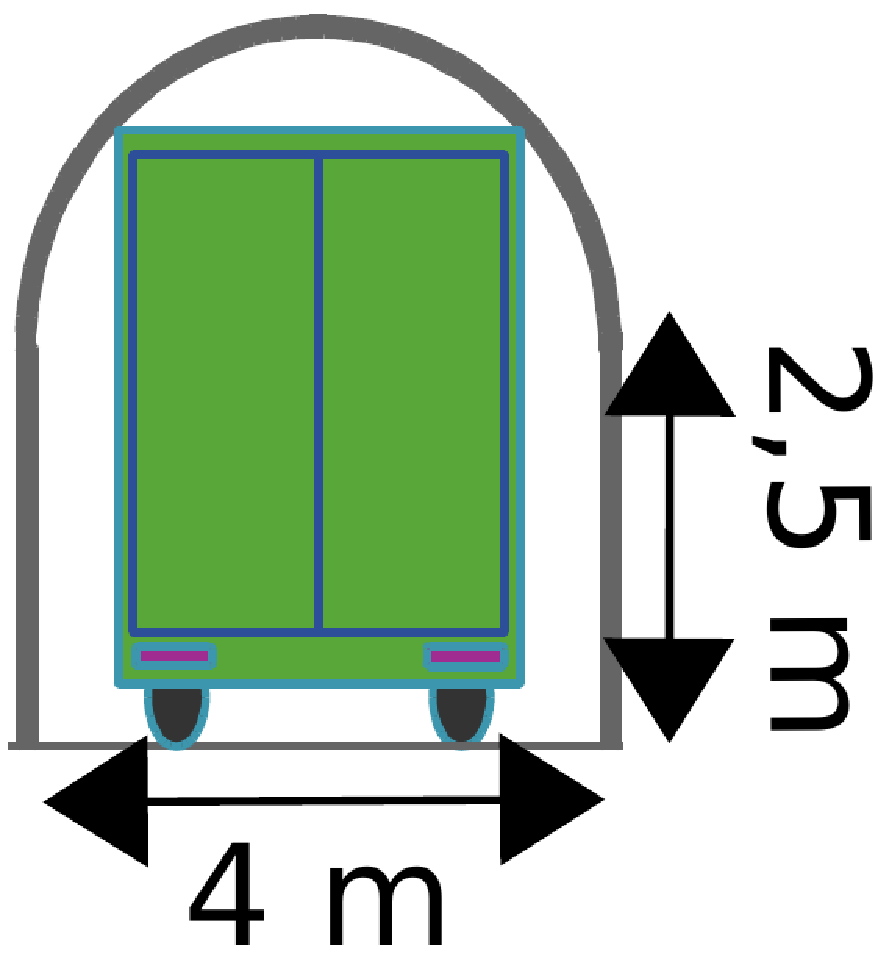
\includegraphics[width=5cm]{camiontunel.pdf}

\corrref{2smath-0264}
\end{exercice}
